\documentclass{scrartcl}
\usepackage[utf8]{inputenc}
\usepackage{amsmath,amssymb,amstext}
\usepackage{mathtools}
\usepackage{hyperref}
\usepackage{graphicx}

\usepackage[onehalfspacing]{setspace}

\begin{document}
	
	\title{Energy Online}
	\subtitle{}
	\author{J. Shah, M. Jordi, M. Stemmle, S. Oeschger, S. Zemljic}
	
	\maketitle
	\section{Introduction - Michael J. - around 600 words}
	
	\subsection{Context}
	
	\paragraph{}
	 The BIOTS program exists to push education for innovative new technologies into universities to help Switzerland o become one of the leading hubs in Blockchain and IoT space.\footnote{Source: \url{http://biots.org/about/}}
	 
	\paragraph{}
	Since 2016, every year the BIOTS program offers three major verticals for the students to build their ideas and use-cases. In 2018, the focus was on sustainability issues, which are currently on the agenda of the UN or hot topics in industry. Challenges from the sponsors Elektrizitätswerk der Stadt Zürich (EWZ), UBS Group AG (UBS), the European founded project FuturICT 2.0 (\url{https://futurict2.eu}) across the following verticals were presented and solved in the program:
	
	\begin{figure} [h]
		\centering
		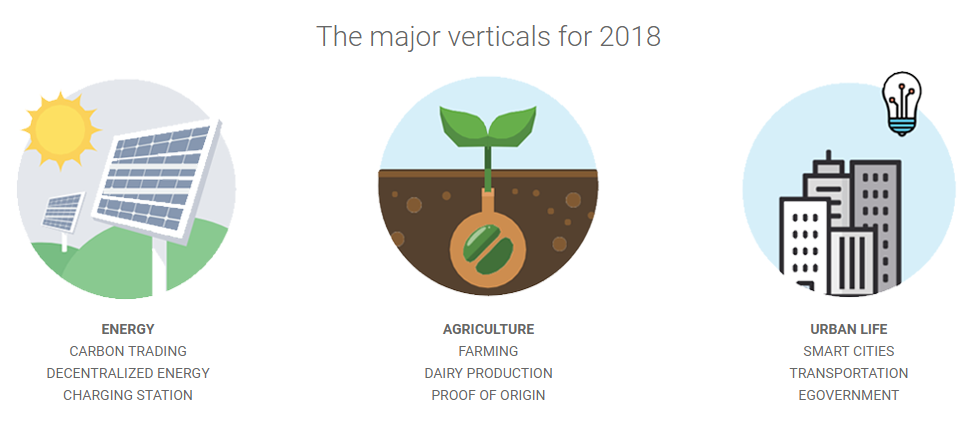
\includegraphics[width=100mm,scale=0.5]{01_introduction_picture01.PNG}
		\caption{Major verticals of BIOTS 2018 , Source \url{http://biots.org/the-biotsphere/}}
	\end{figure}

	\paragraph{}
	This report was created as a result of the challenge 3 “virtual energy storage” from EWZ.
	
	\subsection{Background}
	
	\paragraph{}
	In a cantonal vote 2017 it has been decided, that EWZ needs to sell all its holding in the nuclear sites of Gösgen and Leibstadt until 2034. In addition, EWZ will not be allowed to obtain nuclear energy anymore as well.\footnote{Source: \url{https://www.nzz.ch/zuerich/aktuell/abstimmungssonntag-zuerich-atomausstieg-zuerich-ld.130738}}
	
	\paragraph{}
	In 2016 32.8\% of the electricity in Switzerland is provided by nuclear power plants.\footnote{Source: Schweizerische Elektrizitätsstatistik 2016, p. 5: \url{http://www.bfe.admin.ch/php/modules/publikationen/stream.php?extlang=de\&name=de_306571764.pdf}} To be able to cover those losses, massive investments into renewable energy are needed. Large power plants alone will not be enough to cover the demands, thus small-scale energy production, like private PV's will play a huge role.
	
	\paragraph{}
	Currently, the entry barriers for the installation of PV are high, batterie storage for surplus energy is expensive and overall incentives are missing. For example, energy surplus from private power plants (mainly PV) can only be sold to local energy provider for a very low price of 8.50 Rp./kWh (high tariff) or 4.45 Rp./kWh (low tariff).\footnote{Source: \url{https://www.ewz.ch/content/dam/ewz/services/dokumentencenter/energie-produzieren/dokumente/verguetung-stromruecklieferung-zh-2016-18.pdf)}} To incentivize the installation of PV, promotional money is lacking.\footnote{Source: \url{https://www.srf.ch/news/schweiz/abstellgleis-solarenergie-wer-foerdergelder-will-muss-jahre-warten}}

	\paragraph{}
	To reach the goal of 0\% nuclear energy it is important to make private power plants more lucrative. Therefore, the challenge 3 of EWZ deals with the topic "Virtual Energy Storage". Virtual Energy Storage allows private household to store their surplus energy virtually and withdraw it later when needed.
	
	\paragraph{}
	This concept has been already adapted   Companies like eOn or SENEC already offer services like this to their customers:
	
	\paragraph{}
	eOn (\url{https://www.eon-solar.de/eon-solarcloud})
	
	\begin{itemize}
		\item Service Name:	E.ON SolarCloud
		\item Value Proposition: Genießen Sie jetzt Ihre Sonnenenergie 365 Tage, und Nächte
		\item Value Chain: E.ON -> End customer
		\item Revenue Model: Monthly Fee
		\item Customer Segment: Private Households with PV installations
	\end{itemize}
	
	\paragraph{}
	Senec-ies (\url{https://www.senec-ies.com/tarife-services/senec-cloud/})
	
	\begin{itemize}
		\item Service Name: SENEC.Cloud 2.0
		\item Value Proposition: Strom im Sommer einfrieren und im Winter wieder auftauen.
		\item Value Chain: SENEC -> End customer
		\item Revenue Model: Monthly Fee
		\item Customer Segment:	Private Households with PV installations
	\end{itemize}

	\paragraph{}
	Due to the companies and customers are thrusted parties in those two services offerings, the necessity of the blockchain technology is not given. According to Karl Wüst and Arthur Gervaisy, “Blockchain is being praised as a technological innovation which allows to revolutionize how society trades and interacts. This reputation is in particular attributable to its properties of allowing mutually mistrusting entities to exchange financial value and interact without relying on a trusted third party. A blockchain moreover provides an integrity protected data storage and allows to provide process transparency.”\footnote{“Do you need a Blockchain?”, Karl Wüst, Arthur Gervaisy, \url{https://eprint.iacr.org/2017/375.pdf}}
	
	\subsection{Problem Statement}
	
	\begin{figure} [h!]
		\centering
		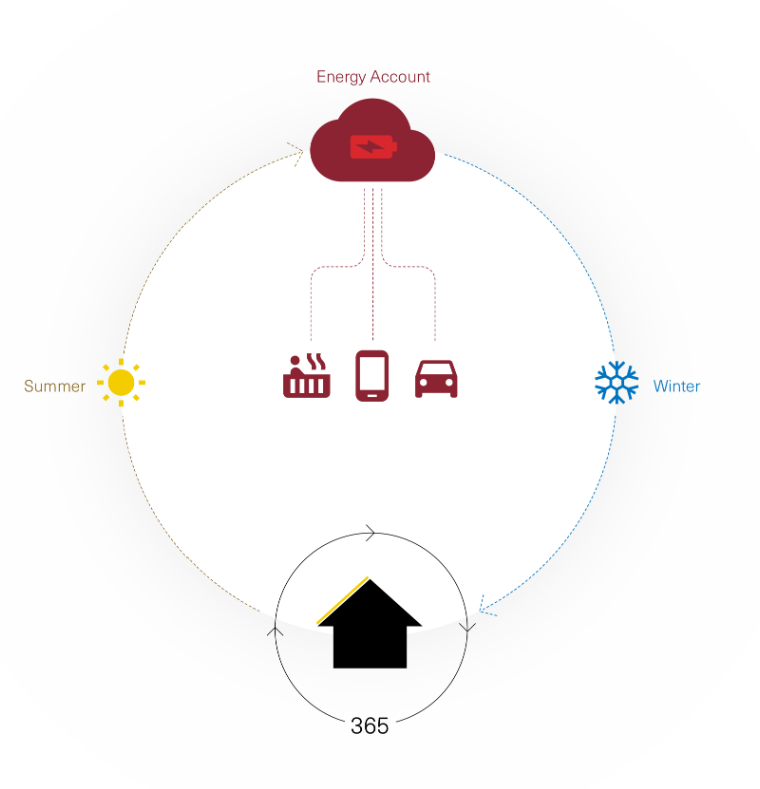
\includegraphics[width=80mm,scale=0.5]{01_introduction_picture02.PNG}
		\caption{EWZ Challenge 3 - "Virtual Energy Storage", Source: \url{BIOTS_ewz_challenges.pdf}}
	\end{figure}
	
	The problem statement given by the EWZ Challenge 3 “Virtual Energy Storage” is: "How might the blockchain technology help to develop a reliable and highly efficient virtual energy solution that gives anyone the possibility to produce, store and use his/her own energy anywhere and anytime? "\footnote{Source: “\url{BIOTS_ewz_challenges.pdf}”}
	
	\section{Literature Review - Jig - around 1100 words}
    
    \begin{itemize}
    \item Business Model https://www.eon-solar.de/eon-solarcloud
    \item Business Model https://www.senec-ies.com/tarife-services/senec-cloud/
    \item Certificats: http://www.bfe.admin.ch/themen/00612/00614/index.html?lang=en
    \item Blockchain and Energy https://hbr.org/2017/03/how-utilities-are-using-blockchain-to-modernize-the-grid
    \item Blockchain and Energy https://www.etla.fi/wp-content/uploads/ETLA-Working-Papers-43.pdf
    \item Blockchain and Energy http://ieeexplore.ieee.org/abstract/document/7589035/
    \item .........
    \end{itemize}
	
	\section{Conceptual Model - Simon around 1100 words - Michael J. around 500 words}
	\subsection{Content}
    \paragraph{}
    Please check https://github.com/StefanOnGit/EnergyOnline/tree/master/report.

    
    \section{Solution Design - Stefan - around 1100 words}
   
    \begin{itemize}
    \item Coding: Architecture, modules etc.- around 900 words .
    \item Evaluation: Features, Bugs etc. - around 200 words
    \end{itemize}
	
    \section{Conclusion/Outlook - Michael S. - around 600 words}
	\paragraph{}
	A very important part are reliable measurements of energy production and consumption. It would be ideal, if smart meters could provide the data directly to the network. But it's highly possible that this does not work yet. As the trust in ewz is very high, and they already check energy consumption manually, this is a service ewz might provide.
	
    \paragraph{}
	Another problem might be on the legal front. The DAO is still a young concept with no laws existing yet. There is also the question, of how the certificates are handled in such a system.  
    
\end{document}